En los ejemplos anteriores se ha evaluado la precisión del método de Taylor con y sin el transporte de jets. Hemos estudiado casos hamiltonianos en donde las soluciones a las ecuaciones diferenciales viven en curvas de energía constante sobre el espacio fase. Es importante tener en cuenta que éste es sólo un subconjunto de casos en la familia de sistemas de ecuaciones diferenciales ordinarias. Nuevos elementos aparecen en los campos vectoriales impuestos por la forma más general de (\ref{eq:ode}) como órbitas periódicas, atractores, repulsores o atractores extraños \cite{Perez2015}. La idea de los indicadores dinámicos radica en encontrar estructuras que nos permitan catalogar a los campos vectoriales, sean hamiltonianos o no, y sacar información relevante acerca de las soluciones al sistema de ecuaciones dado. 

Hay que destacar que el transporte de jets no sirve únicamente para dar indicadores dinámicos del espacio fase. Hay un montón de cosas que se pueden aprovechar al tener la solución parametrizada por polinomios. Entre éstas están hacer simulaciones de Montecarlo o hacer variación de los parametros de las ecuaciones.

\subsection{Un poco de motivación vía exponentes de Lyapunov}

El transporte de jets es relevante en el sentido de poder hacer variaciones de tamaño $\delta x$ alrededor de $\xo$ y ver cómo evoluciona el flujo $\flowU$ de toda la vecindad $\Uxo$ en el tiempo. Respecto a esto, son conocidos los esfuerzos realizados por saber qué pasa en la vecindad de una condición inicial $\xo$ bajo la aproximación lineal del campo vectorial que define su trayectoria. Surge de aquí la idea de los \textit{Exponentes de Lyapunov a Tiempo Finito}, o ELTF, que busca encontrar cómo se separan dos soluciones cercanas dadas por las trayectorias de $\xo$ y la aproximación lineal de la trayectoria de $\xo + \delta\xo$. Esto permitirá encontrar componentes de caos \cite{Perez2015}, estructuras lagrangianas, separatrices \cite{Perez2015}, ciclos límite, entre otras. 

Sea $\dot{\mathbf{x}}(t) = \mathbf{f}(\mathbf{x}(t),t) = A\mathbf{x}+\mathcal{O}(\mathbf{x}^2)$ un sistema de $d$ grados de libertad que describe un campo vectorial con parte lineal $A \mathbf{x}$. Si nos quedamos únicamente con ésta, podemos encontrar la solución explícita al sistema
\begin{equation*}
 \mathbf{y}(t) = \mathbf{y}_0 e^{\Lambda t}
\end{equation*}

con $\Lambda = [\lambda_i]$ una matriz diagonal con las $d$ raíces del polinomio característico $P(\lambda) = \det(A - \lambda \mathbf{1})$ y $\mathbf{x} = P \mathbf{y}$, con $P = [\mathbf{v_i}]$, la matriz simétrica de $[d \times d]$ de cambio de coordenadas formada por los eigenvectores asociados a $\lambda_i$, $\mathbf{v}_i$.
Dada ésta solución, vemos que las soluciones vecinas son simplemente 
\begin{equation*}
 (\mathbf{y} + \mathbf{\delta y})(t) = (\mathbf{y}_0 + \mathbf{\delta y}_0) e^{\Lambda t}
\end{equation*}

y luego regresar al sistema de coordenadas original bajo $P$\footnote{Buscamos eigenvectores $\mathbf{v}_i$ tales que $\det(P) = 1$, de modo que la transformación $\mathbf{x} = P \mathbf{y}$ preserve área y orientación.}. 

%Valdrá la pena mencionar aquí algo sobre  el ESPECTRO DE LYAPUNOV? Yo creo que sí, ya que, en sistemas hamiltonianos TR(\Lambda) == 1 y, además, habla un poco de cómo se deforman las soluciones linealmente alrededor de un punto en todas las direcciones 

Con lo anterior podemos plantear una forma intuitiva en la que se separan dos soluciones cercanas
\begin{equation}
 \norm{ \mathbf{\delta x}(t) \norm{ = e^{\lambda t} } \mathbf{\delta x}_0 }.
 \label{eq:lyap-sep}
\end{equation}
donde $\lambda$ es el máximo eigenvalor de todos los $\lambda_i$'s de $\Lambda$. Notemos que la variación $\delta x$ debe ser suficientemente pequeña para que $A\mathbf{x}$ sea el término dominante de $f$ aunque, en el límite $\delta x \to 0$, esto es cierto por completo. 

Los ELTF son, en escencia, indicadores escalares que, para cada punto $\mathbf{x}$ del espacio fase, nos dice qué tan grande será la tasa de separación a soluciones cercanas. Estos se obtienen de despejar (\ref{eq:lyap-sep})
\begin{equation}
 \lambda_{\xo}^t = \frac{1}{t}\ln \left( \frac{\norm{\mathbf{ \delta x(t)} }_2}{\norm{ \mathbf{\delta x}_0 }_2} \right)
 \label{eq:lyap-exp}
\end{equation}
y hacer un análisis (lineal) un poco más riguroso sobre las variaciones $\delta \mathbf{x}$.

Es importante resaltar que en los casos donde $\delta \xo$ se aleja de $\xo$ en el tiempo, la separación puede volverse tan grande que la aproximación lineal planteada por (\ref{eq:lyap-sep}) no es válida. Por esto, como se sugiere en \cite{ChaosBook}, es conveniente, dada la separación  $\delta \mathbf{x}(\Delta t_1)$ en un intervalo $\Delta t_1$ donde valga la aproximación lineal, encontrar $\lambda_1 = \lambda_{\xo}^{\Delta t_1}$ para éste intervalo y luego reescalar $\delta \mathbf{x}(\Delta t_1)$ en un factor de $\norm{ \delta \xo / \delta \mathbf{x}(\Delta t_1) }$ para que la magnitud de la separación después de éste intervalo de tiempo sea igual que la inicial $\delta \xo$. Con esto, se puede encontrar el exponente (\ref{eq:lyap-exp}) para tiempos largos con
\begin{equation*}
 \lambda_{\xo}^t = \frac{1}{t} \sum_{i} \Delta t_i \lambda_i
    \quad\text{,}\quad 
 \sum_i \Delta t_i = t
\end{equation*}
evitando así problemas en las no linealidades\footnote{Suena muy lindo pero no es cierto siempre; ver \ref{eq:} } y tomando en cuenta, además, los casos donde $\mathbf{f}(\mathbf{x}(t),t) = A(t)\mathbf{x} + \ldots $, ya que cada exponente $\lambda_i$ se haría en relación a $A(t_i)$.

Sea $\phi: \mathbb{R} \times \mathbb{R} \times \mathcal{D} \to \mathcal{D}$, $\mathcal{D} \subset \mathbb{C}^d$ el flujo de $\dot{\mathbf{x}}(t) = f(\mathbf{x}(t),t)$, donde

\begin{equation*}
 \phi(t;t_0,\xo + \delta \xo) = (\mathbf{x + \delta x})(t) = \phi(t;t_0,\xo) + \sum_{j=1}^d \frac{\partial \mathbf{x}(t)}{\partial \mathbf{x}_{0_j}}\delta \mathbf{x}_{0_j} + ...
\end{equation*}

es la expansión en serie de Taylor de $\phi$ alrededor de $\xo$, entonces 
\begin{equation*}
 \delta \mathbf{x}(t) \approx J^t(\xo) \cdot \delta \xo
\end{equation*}

con 
\begin{equation}
 J^t(\xo) = \frac{\partial \phi(t;t_0,\xo)}{\partial \mathbf{x}_{0}}
 \label{eq:jacobian}
\end{equation}
la matriz jacobiana para $\flowci$ alrededor de $\xo$. Con esto, obtenemos una forma más práctica de obtener los ELTF
\begin{equation}
 \lambda_{\xo}^t = \frac{1}{t}\ln \left( \norm{J^t(\xo) }_2 \right)
\end{equation}
ya que, por la construcción del álgebra polinomial, podemos calcular $J^t(\mathbf{x})$ para cada paso de una integración de jets en polinomios de orden $M=1$ y obtener, naturalmente, los ELTF.

En el caso de dos grados de libertad\footnote{El caso de $d$ grados de libertad es idéntico y más aparatoso en notación y, por tanto, no lo voy a hacer.}, el flujo obtenido al integrar alrededor de $P_{0,\xo} = (x_{1_0} + \xi_1, x_{2_0} + \xi_2 )^T$ al tiempo $t=t_n$ se ve como $P_{n,\xo} = (x_1(t_n) + \alpha_1^{(n)} \xi_1 + \beta_1^{(n)} \xi_2, x_2(t_n) + \alpha_2^{(n)} \xi_1 + \beta_2^{(n)} \xi_2)^T$ y, por tanto, 

\begin{align}
 J^{t_n}(\xi) = \left[ \begin{array}{ccc}
 \alpha_1^{(n)} & \beta_1^{(n)}  \\
 \alpha_2^{(n)} & \beta_2^{(n)}
 \end{array} \right].
 \label{eq:jac_jt}
\end{align}

Geométricamente, (\ref{eq:jac_jt}) representa la deformación lineal de una variación $\delta \mathbf{x}$ respecto de $\xo$ para cada paso en $t$ donde, para $t = t_0$, $J^0(\xi) = \mathbf{1}$.

%Detalles técnicos para "computar" el campo de ELTFs; grid de puntos, qué se calcula, etc 

%FIGURA!
\begin{figure}[h!]
 \centering
 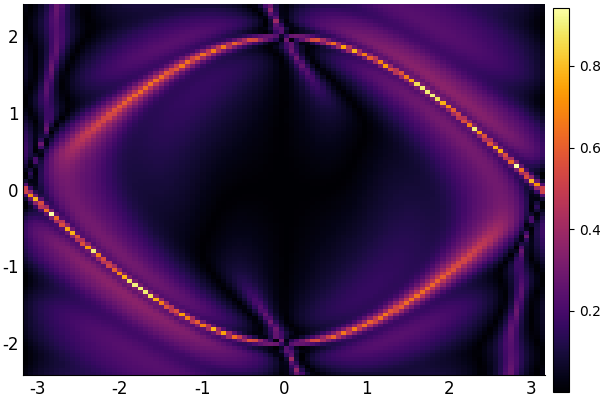
\includegraphics[width=0.7\linewidth]{ftle_pendulum}
 \caption{Campo escalar de los ELTF para el péndulo de (\ref{eq:pendulo-ode}) en una retícula de $100$ puntos por lado, después de un periodo, con tolerancia $\epsilon_{Taylor} = 10^{-10}$ y orden máximo de la expansión $M = 25$.}
 \label{fig:ftle_pendulum}
\end{figure}

En la figura \ref{fig:ftle_pendulum} podemos ver el campo escalar de los ELTF calculados a partir de (\ref{eq:lyap-exp}) para el péndulo simple descrito por (\ref{eq:pendulo-ode}). Es interesante notar cómo éste percibe, por llamarlo de alguna manera, la presencia de separatrices en el espacio fase, ya que en estas las soluciones cercanas se alejan mucho de la separatriz. En \cite{Haller2011}, se hace un análisis profundo sobre detectar diferentes regiones en el espacio fase, que ahí las llama \textit{Estructuras Lagrangianas Coherentes}, motivado en la parcelas lagrangianas de la mecánica de fluidos. Como se muestra en la referencia anterior, no necesariamente el campo escalar de ELTF va a encontrar separatrices, sino puntos cuyas soluciones vecinas se alejan rápidamente en el tiempo; esto puede indicar, sí, separatrices, pero también caos, o grandes gradientes de velocidad en el espacio fase.
%Un par más de ejemplos

Hemos visto cómo el campo escalar de ELTF proporciona un buen indicador de la estructura de los campos vectoriales en relación con qué pasa linealmente en la vecindad de diferentes puntos del espacio fase. Sin embargo, existen casos donde éste no es suficiente para entenderlos o clasificarlos. 

%Casos donde esto falla o donde el jacobiano no es suficientemente buena aproximación... 

\subsection{Tamaño máximo de las vecindades}

Vimos, en el caso anterior, cómo el jacobiano $J^{t_n}(\xi)$ representa la deformación lineal de las trayectorias vecinas a $\xo$ al tiempo $t_n$ y cómo, con éste, se puede calcular el campo escalar de los ELTF. Sin embargo, en los ejemplos XXX se observa que a veces la aproximación lineal de las deformaciones no es suficiente para sacar conclusiones contundentes sobre el sistema de EDO. De hecho, por el teorema de Grobman-Hartman, existen casos donde las ecuaciones no son siquiera topológicamente equivalentes a su aproximación lineal. 
%Trabajar los ejemplos XXX.

Para el TJ no tenemos, a priori, la restricción de la linealidad. Lo único que se hizo para adaptar el TJ al campo de ELTF fue tomar una expansión a primer orden de las soluciones de un campo vectorial dado. Sin embargo, si las expansiones de los polinomios son de orden $N > 1$, entonces las deformaciones en las vecindades de $\xo$ exhibirán términos no lineales para cada término del flujo y, así, se puede obtener información más precisa en los indicadores pertinentes\footnote{La figura \ref{fig:pendulum_jt} es un buen ejemplo de cómo no siempre las deformaciones lineales son suficientes.}. Intuitivamente, entre mayor sea el orden de expansión de los jets, mejor será la aproximación a la solución real en las vecindades de $\xo$; sin embargo, no se ha analizado \textit{que tan grandes} deben ser dichas variaciones para estar bajo una tolerancia controlada.

%FIGURA!
\begin{figure}[h!]
	\centering
	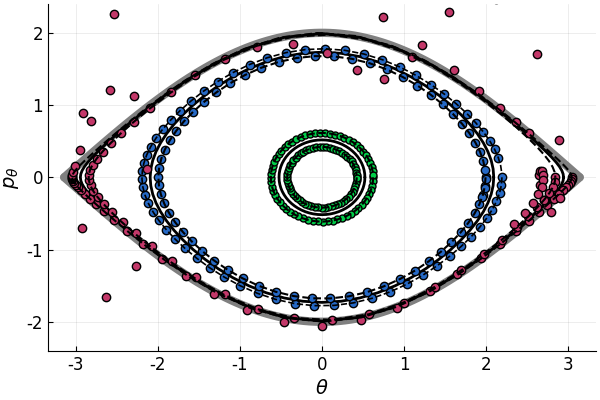
\includegraphics[width=0.7\linewidth]{xi_precision_pendulum}
	\caption{Diferencia de energía $\delta E(t_n) = \frac{1}{\epsilon_{machine}} \left( H(\mathbf{x}(t_n)) - H(\xo) \right)$ para el sistema (\ref{eq:artificial_ode}) con jets de orden $M=16$ evaluados en $\xi_{max} = 0.0235$, el cual se calculó con $\epsilon_{jet} = 10^{-14}$. Se utilizó tolerancia $\epsilon_{Taylor} = 10^{-10}$, orden de expansión $N = 25$ y $40$ pasos temporales de $t_0 = 0$ a $t_{max} = 1.7$.}
	\label{fig:xi_precision_pendulum}
\end{figure}

%FIGURA! 
%\begin{figure}[h!]
%\centering
%\begin{subfigure}{0.49\textwidth}
%	\centering
%	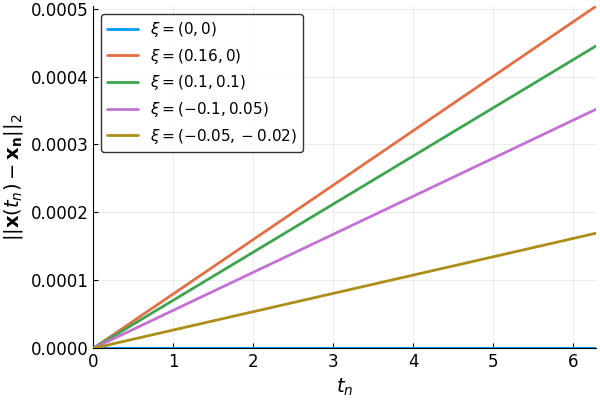
\includegraphics[width = \textwidth]{euler-vs-analytical_center}
%	\caption{Norma de la diferencia entre la solución real y evaluaciones de la solución numérica para distintos valores de $\xi$ marcados en la gráfica. Se puede observar un crecimiento lineal del error numérico, lo cual es una de las consecuencias de usar el método de Euler.}
%	\label{fig:center-eu_vs_anal}
%\end{subfigure}
%%
%\begin{subfigure}{0.49\textwidth}
%	\centering
%	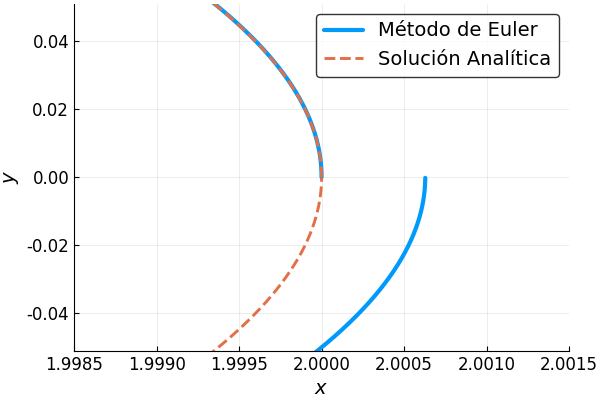
\includegraphics[width = \textwidth]{euler-method_error}
%	\caption{Sección del espacio fase donde se observan la solución analítica y la solución numérica para pasos de $h=10^{-4}$ con cóndición inicial $\xo = (2,0)$. \\ \\}

Suponiendo que la expansión en series de $\flowxi$ corresponde a una expansión analítica, los coeficientes de la expansión irán convergiendo en cuanto crezca el orden. Así, una forma de controlar qué tan grandes pueden ser las variaciones alrededor de $\xo$ es acotar la contribución del último término a una tolerancia dada; es decir,
\begin{equation*}
 a_{M}^{(n)}\xi_{max}^M \leq \epsilon_{jet}
\end{equation*}
donde $\flowxi = P_{n,\xo}(\xi) = \sum_{|m|=1}^M  a_{m}^{(n)} \xi^m$, con $a_{m}^{(n)}$ el polinomio de orden $m = \norm{\mathbf{m}}_1$ del jet al tiempo $t_n$.

Se busca controlar el máximo de estos coeficientes, de modo que 
\begin{align}
 \xi_{max} = \min_{|m|=M} \left( \frac{\epsilon_{jet}}{a_{m}^{(n)}} \right)^{\frac{1}{m}}.
\end{align}
es el radio máximo que la vecindad $\Uxo$ puede tomar para estar debajo de la tolerancia controlada. 

Con ésto se establece qué tan grandes pueden ser las variaciones de $\xo$ sin que las deformaciones del jet repercutan de manera drástica en las soluciones evaluadas. La sección \ref{sec:artificial_ham} muestra cómo la dinámica del campo vectorial exige que las deformaciones de $\Uxo$ sean muy grandes y, como se observó en la figura \ref{fig:artificial_dEjets_all}, después de cierto tiempo la energía deja de conservarse, lo cual implica que la solución ya no vive en la curva de nivel del hamiltoniano y, por tanto, el TJ no es suficiente preciso para determinar soluciones cercanas o, visto de otro ángulo, la vecindad en la que se evaluó era demasiado grande para conservar la energía en toda la trayectoria del flujo.

%FIGURA!
\begin{figure}[h!]
	\centering
	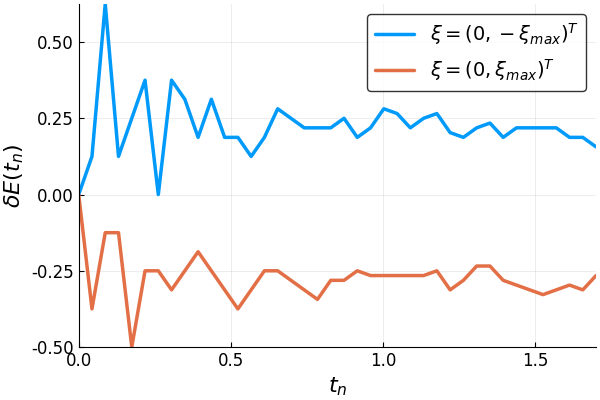
\includegraphics[width=0.7\linewidth]{dE_ximax_ah}
	\caption{Diferencia de energía $\delta E(t_n) = \frac{1}{\epsilon_{machine}} \left( H(\mathbf{x}(t_n)) - H(\xo) \right)$ para el sistema (\ref{eq:artificial_ode}) con jets de orden $M=16$ evaluados en $\xi_{max} = 0.0235$, el cual se calculó con $\epsilon_{jet} = 10^{-14}$. Se utilizó tolerancia $\epsilon_{Taylor} = 10^{-10}$, orden de expansión $N = 25$ y $40$ pasos temporales de $t_0 = 0$ a $t_{max} = 1.7$.}
	\label{fig:dE_ximax_ah}
\end{figure}

En la figura \ref{fig:dE_ximax_ah} retomamos al sistema \ref{eq:artifical_ode} que, en su momento, vimos cómo su energía divirgió; ahora podemos ver que, al establecer una tolerancia $\epsilon_{jet} = 10^{-14}$, las variaciones de energía para ambos casos $\pm \xi_{max}$ son \textbf{más pequeñas que el épsilon de la máquina}. Esto implica que establecer un tamaño máximo de las vecindades reduce drásticamente el error de las soluciones calculadas. Esto, sin embargo, tiene un costo relativamente alto, ya que $\xi_{max} = 0.0235 \ll 0.1$, donde $0.1$ fue la variación respecto a $\xo$ que se había escogido aleatoriamente en la sección \ref{sec:benchmark-taylor}. 

$\xi_{max}$ depende fuertemente de la tolerancia $\epsilon_{jet}$ escogida y, más importantemente, de la condición inicial en donde se busque saber la variación máxima posible. En general, entre más se deforme el jet con la evolución del flujo, menores serán las vecindades en las que las evaluaciones de $\flowxi$ queden debajo de $\epsilon_{jet}$. Con esto en mente, el tamaño máximo de la vecindad puede servir como un indicador similar a los ELTF, ya que es sensible a la separación entre condiciones iniciales cercanas. El tamaño de vecindad va a detectar grandes gradientes de velocidades, presencia de separatrices en el espacio fase y regiones de caos en \textbf{órdenes no lineales de la vecindad de las soluciones}. Se muestra en la figura \ref{fig:jt_ximax_ah} cómo $\flowU$ consta de una $\Uxo$ considerablemente más pequeña que en \ref{fig:artificial_jt}.

%FIGURA!
\begin{figure}[h!]
 \centering
 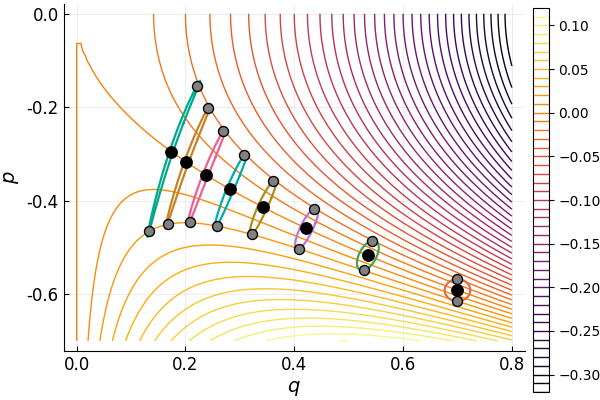
\includegraphics[width=0.7\linewidth]{jt_ximax_ah}
 \caption{Solución para (\ref{eq:artificial_ode}), con condición inicial sobre la separatriz, donde $q_0 = 0.7$. Aquí, los jets son de orden $M=16$, en $8$ pasos de integración desde $t_0 = 0$ hasta $t_{max} = 1.7$, evaluados para $\xi_{max} = 0.025$. Se utilizó tolerancia $\epsilon_{Taylor} = 10^-{20}$ y orden de la expansión $N=25$. En gris están las soluciones a $\xo \pm \xi_{max}$ sin utilizar TJ.}
 \label{fig:jt_ximax_ah}
\end{figure}

Dicho lo anterior, y a modo de comparar con los ELTF desarrollados previamente, tomemos el caso del péndulo simple, que tiene una separatriz que divide la zona en donde el péndulo oscila respecto a un punto de equilibrio (`` '') y la zona donde el péndulo completará períodos completos de oscilación (``libración'') . A diferencia de la figura \ref{fig:ftle_pendulum}, la figura \ref{fig:ximax_pendulum} alcanza sus mayores valores en el centro, que es donde las velocidades del campo vectorial son menores y, en cambio, en los valores de la separatriz, se alcanzan los mínimos valores para $\xi_{max}$, ya que es donde los jets sufren mayores deformaciones. Sin embargo, ésta figura nos da información equivalente a los ELTF, ya que, cualitativamente, presenta la misma información y nos indica sobre la presencia de la separatriz. 

%FIGURA!
\begin{figure}[h!]
 \centering
 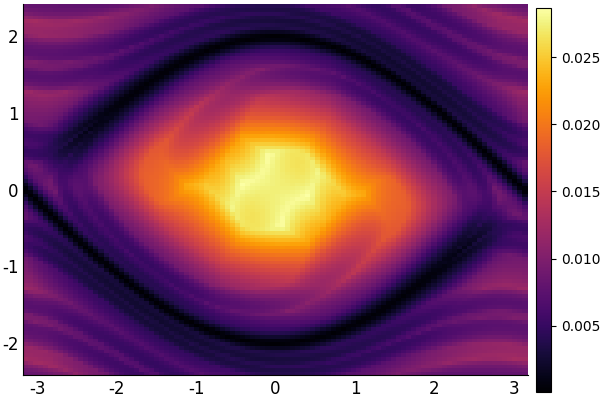
\includegraphics[width=0.7\linewidth]{ximax_pendulum}
 \caption{Campo escalar de los tamaños máximos de vecindad $\xi_{max}$ para el péndulo de (\ref{eq:pendulo-ode}) en una retícula de $60$ puntos por lado, después de un periodo, con tolerancia $\epsilon_{Taylor} = 10^{-10}$ y orden máximo de la expansión $M = 25$.}
 \label{fig:ximax_pendulum}
\end{figure}

%Hacer más ejemplo(s) con esto

\subsection{Tasa de expansión y contracción}
\label{sec:contraccion_expansion}

Otra forma de obtener información sobre los flujos es viendo la tasa de deformación de los jets propagados en el espacio fase. La ventaja de esto sobre el campo escalar de ELTF o del tamaño máximo de vecindades es que aquí es posible saber \textbf{en qué dirección} se tienen la mayor y menor deformación respecto a un punto en el espacio fase. Este indicador se relaciona, en este sentido, con el espectro de Lyapunov, que no es más que el conjunto de eigenvalores $\lambda_i$ obtenidos por las raíces del polinomio característico $P(\lambda) = \det(A - \lambda\mathbf{1})$. El espectro de Lyapunov nos dice cómo crece o se contrae la aproximación lineal de las soluciones bajo un cambio invertible de coordenadas. Las \textbf{tasas de expansión y contracción} de vecindades del flujo $\flowci$ ($\zeta_+$ y $\zeta_-$, respectivamente) nos dicen cuáles son la máxima y mínima separación de $\xo$ con una variación $\xi$ de radio $|\xi(\theta)| = \xi_{max}$.

Para obtener dicho indicador se hace el TJ del orden $M$ deseado integrando hasta $t = t_n$, se obtiene el radio máximo de la vecindad con el método de la sección anterior y se evalúa la frontera de $\Uxo$ en $P_{n,\xo}(\xi(\theta))$. Una vez evaluada, se encuentra el ángulo de máxima (mínima) separación 
\begin{equation}
 \theta_{+}(\xo) = \max_{\theta \in [0,2\pi)} \norm{ P_{n,\xo}(\xi(\theta)) - P_{n,\xo}(0) }
\end{equation} 
y se calcula 
\begin{equation}
 \zeta_{\pm}(\xo) = \frac{ \norm{P_{n,\xo}(\xi(\theta_{\pm})) - P_{n,\xo}(0)} }{\xi_{max}}.
 \label{eq:max_min_rate}
\end{equation}

En el caso de dos grados de libertad, como los ejemplos hasta ahora planteados, se ha parametrizado dicha frontera con $\xi(\theta) = \xi_{max} \left( \cos(\theta), \sin(\theta) \right)^T, \theta \in [0,2\pi]$. Evidentemente no se puede evaluar la frontera de $\Uxo$ en un continuo de puntos en la computadora, así que se plantean dos maneras de mejorar la precisión sobre dichos máximos y mínimos: 
\begin{itemize}
\item Aumentar el número de puntos con los cuales se evalúa $\delta \Uxo$
\item Encontrar $\theta_{\pm}$ de los puntos disponibles y luego hacer un Newton-Rapson con $P_{n,\xo}$. 
\end{itemize} 

Se pueden encontrar $\theta_\pm$ y $\zeta_\pm$ para todo una rejilla de puntos y obtener dos campos vectoriales y dos escalares, respectivamente. Los campos vectoriales indican, para cada punto, la dirección de mayor y menor separación de la condición $\xo$ dada; los campos escalares indican la magnitud de esto último. En la figura \ref{fig:seprate_pendulum} se pueden ver ambos campos encimados para el péndulo simple donde, para cada punto de la rejilla, hay un vector en la dirección de máxima (mínima) separación y en color se indica la magnitud de dicha separación.

%FIGURA! 
\begin{figure}[h!]
\centering
\begin{subfigure}{0.49\textwidth}
	\centering
	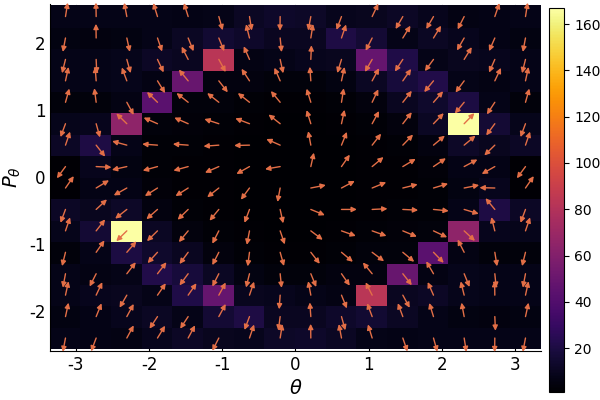
\includegraphics[width = \textwidth]{seprate_max_pendulum}
	\caption{Campos vectorial y escalar calculados con $\theta_+(\xo)$ y $\zeta_+(\xo)$,respectivamente.}
	\label{fig:seprate_max_pendulum}
\end{subfigure}
%
\begin{subfigure}{0.49\textwidth}
	\centering
	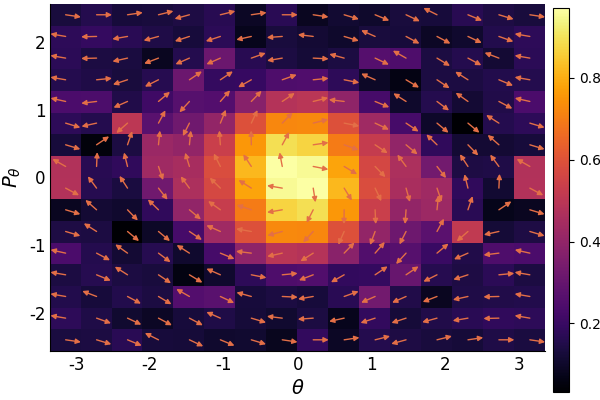
\includegraphics[width = \textwidth]{seprate_min_pendulum}
	\caption{Campos vectorial y escalar calculados con $\theta_-(\xo)$ y $\zeta_-(\xo)$,respectivamente.}
	\label{fig:seprate_min_pendulum}
\end{subfigure}
\caption{ Campos vectoriales dados por $\left( \cos(\theta_\pm(\xo)),\sin(\theta_\pm(\xo)) \right)^T$ sobre los campos escalares $\zeta_\pm(\xo)$ para el péndulo simple, en rejillas de $15\times15$, con tolerancia $\epsilon_{Taylor} = 10^{-20}$, orden de los jets $M=3$ y orden de la expansión $N=25$. }
\label{fig:seprate_pendulum}
\end{figure}

Es curioso ver que, para los campos escalares de $\zeta_\pm$, se detecta la presencia de la separatriz en un modo similar que en las dos subsecciones anteriores. De hecho, $\zeta_\pm$ puede utilizarse también como un indicador de separatrices, caos y grandes gradientes de velocidad. La figura \ref{fig:seprate_scalar_pendulum} nos muestra una versión más refinada de los campos escalares correspondientes.\footnote{Se toma la raíz cúbica de $\zeta_\pm$ para achicar la diferencia entre los valores máximos y mínimos y que la imagen sea más legible.} 

%FIGURA!
\begin{figure}[h!]
\centering
\begin{subfigure}{0.49\textwidth}
	\centering
	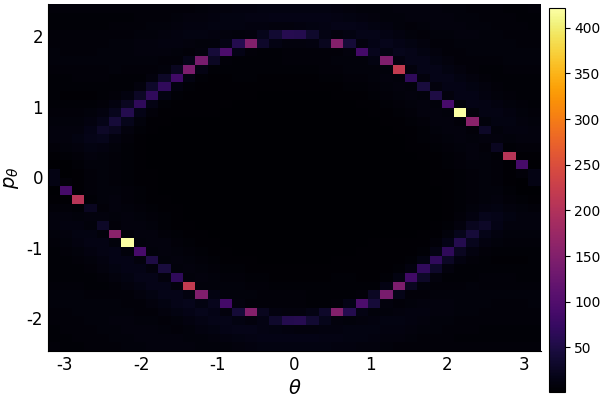
\includegraphics[width = \textwidth]{seprate_max_scalar_pendulum}
	\caption{Campo escalar $\zeta_+(\xo)$.}
	\label{fig:seprate_max_scalar_pendulum}
\end{subfigure}
%
\begin{subfigure}{0.49\textwidth}
	\centering
	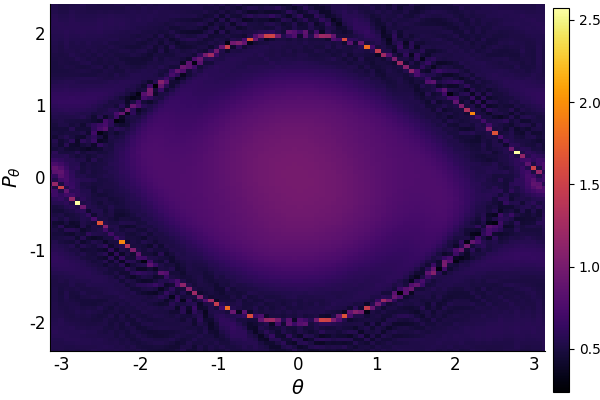
\includegraphics[width = \textwidth]{seprate_min_scalar_pendulum}
	\caption{Campo escalar $\zeta_-(\xo)$.}
	\label{fig:seprate_min_scalar_pendulum}
\end{subfigure}
\caption{ Campos escalares $\left( \zeta_\pm(\xo) \right)^{1/3}$ para el péndulo simple, en rejillas de $90\times 90$, con tolerancia $\epsilon_{Taylor} = 10^{-20}$, orden de los jets $M=3$ y orden de la expansión $N=25$. }
\label{fig:seprate_scalar_pendulum}
\end{figure}

%Teniendo xi_max se puede ver en qué dirección se expande más (menos) la deformación de de dx. ESte se hace encontrando el máximo y mínimo en la vecindad evaluada. ¿Cómo serviría esto? 

\subsection{Formas Simplécticas}
\label{sec:formas-simplecticas}
%Motivar un poco porqué hablaríamos de formas simpléticas y decir que el desarrollo viene motivado del chaosbook... si se puede encontrar algún otro libro para complementar estaría muy bien. 

Tenemos, de (\ref{eq:hamiltonian}), que
\begin{align*}
H: \mathcal{M} \subset \mathbb{R}^d\times\mathbb{R}^d &\to \mathbb{R} \\ 
	(\mathbf{q},\mathbf{p}) &\to H(\mathbf{q},\mathbf{p})
\end{align*}

es el hamiltoniano que define al sistema de ecuaciones diferenciales ordinarias

\begin{align*}
 \dot{\mathbf{q}} &= \ \pder{H}{\mathbf{p}} \\
 \dot{\mathbf{p}} &= - \pder{H}{\mathbf{q}}. 
\end{align*}

Si definimos $\mathbf{x} := (\mathbf{q},\mathbf{p}) = (x_1,\ldots,x_{2d})^T$, entonces
\begin{equation}
 \dot{x_i} = \omega_{i,j} \pder{H(\mathbf{x})}{x_j}
 \label{eq:symplectic_ham_ode}
\end{equation}

donde
\begin{equation}
 \omega = 
    \begin{bmatrix}
    \mathbf{0} & \mathbf{I} \\
    -\mathbf{I} & \mathbf{0}
  \end{bmatrix}
 \label{eq:symplectic_omega}
\end{equation}

es una matriz de $2d\times 2d$, $\mathbf{0}$ es una matriz de ceros de $d\times d$ y $\mathbf{I}$ es la matriz identidad de $d\times d$. Notemos que (\ref{eq:symplectic_omega}) cumple
\begin{align}
 \omega^2 &= -\mathbf{I}  \nonumber \\
 \omega^T &= -\omega
 \label{eq:omega_properties}
\end{align}
para cualquier $d$.

\begin{definicion}
Sea $\omega$ una matriz que cumple las propiedades (\ref{eq:omega_properties}). Se dice que una matriz $g$ es \textbf{simpléctica} si
\begin{equation}
 g^T \omega g = \omega.
 \label{eq:symplectic_condition}
\end{equation}
%Ver lo de las formas bilineales... Posiblemente se pueda partir de una definición más formal/general y concluir esto para g. 
\end{definicion}

Las matrices que cumplen la definición anterior forman un \textbf{grupo simpléctico} denotado $Sd(d)$, que son un caso particular de los grupos de Lie.

Los \textbf{grupos de Lie} son grupos cuyos elementos dependen de un número finito de parámetros, i.e., $g = g(\eta) = g(\eta_1,\ldots,\eta_N)$. Dicho esto, y como se menciona en \cite{ChaosBook}, para los cálculos se suele escoger una base para operar dichas matrices y, para transformaciones infinitesimales del espacio fase, éstas toman la forma
\begin{equation}
 g(\delta \eta) := \mathbf{1} + \delta \eta \mathbf{T}
 \label{eq:symp_infinit_rotation}
\end{equation}

con $\lbrace T_1, \ldots, T_N \rbrace$ un conjunto de rotaciones\footnote{Dichas rotaciones representan las deformaciones infinitesimales de las transformaciones de $g$.} sobre el espacio fase.

Notemos que si al grupo de rotaciones (\ref{eq:symp_infinit_rotation}) le imponemos la condición (\ref{eq:symplectic_condition}) de simplecticidad

\begin{align*}
  \left( \mathbf{1} + \delta \eta \mathbf{T} \right)^T \omega \left( \mathbf{1} + \delta \eta \mathbf{T} \right) = \omega \implies 
  \cancel{\omega} + (\delta \eta \mathbf{T})^T \omega + \omega \delta \eta \mathbf{T} + \cancelto{\mathcal{O}(\norm{\delta \eta \mathbf{T}}^2)} {(\delta \eta \mathbf{T})^T \omega \delta \eta \mathbf{T}} = \cancel{\omega}  
\end{align*}

obtenemos una forma explícita para que éste sea simpléctico
\begin{equation}
  (\delta \eta \mathbf{T})^T \omega + \omega \delta \eta \mathbf{T} = \mathbf{0}.
  \label{eq:eq:symplectic_condition2}
\end{equation}

En el caso de tener un hamiltoniano $H(\mathbf{x})$, basta darse cuenta que
\begin{itemize}
\item $H(\mathbf{x})$ es, al menos, $\mathcal{C}^2(\mathcal{M})$; esto es, $\frac{\partial^2 H}{\partial x_i \partial x_j} = \frac{\partial^2 H}{\partial x_j \partial x_i}$.

\item Los generadores de las transformaciones infinitesimales del sistema de EDO (\ref{eq:ode}) están dadas por $A_{i,j}(\mathbf{x}) := \pder{f_i(\mathbf{x})}{x_j}$\footnote{Es importante observar que, como el sistema es hamiltoniano, $f(\mathbf{x}(t),t) = f(\mathbf{x})$.}. $A_{i,j}(\mathbf{x})$ son los elementos de matriz de $A(\mathbf{x})$, la cual se conoce como \textbf{matriz de estabilidad} del sistema.

\item La matriz de estabilidad puede representarse en términos de $\omega$ como $A(\mathbf{x}) = \omega \Xi(\mathbf{x})$, donde $\Xi(\mathbf{x}) = \left[ \frac{\partial^2 H(\mathbf{x})}{\partial x_i \partial x_j} \right]$ es el \textbf{hessiano}, o matriz de segundas derivadas, de $H$.

\item Como $H$ es $\mathcal{C}^2(\mathcal{M})$, entonces $\Xi$ es simétrica y, por tanto, $\Xi = \Xi^T$.
\end{itemize}

Con las observaciones anteriores podemos ver que
\begin{align*}
 A(\mathbf{x})^T \omega + \omega A(\mathbf{x}) = \Xi(\mathbf{x})^T \cancelto{\mathbf{I}}{\omega^T \omega} + \cancelto{-\mathbf{I}}{\omega \omega}\Xi(\mathbf{x}) = \Xi(\mathbf{x})^T - \Xi(\mathbf{x}) = 0.
\end{align*}

Así, cualquier sistema hamiltoniano es un sistema simpléctico y cumple
\begin{equation}
 A^T\omega + \omega A = 0
 \label{eq:symplectic_hamiltonian}
\end{equation}
%Meterlo como corolario o teorema? Chance es más elegante.

%Valdrá la pena hablar/demostrar que la simplecticidad implica la conservación de volumen? 

Regresemos, como siempre, al caso del péndulo simple. Sabemos, por (\ref{eq:pendulo-ham}), que es un sistema hamiltoniano y, por tanto, debe de cumplir (\ref{eq:symplectic_hamiltonian}). La matriz de estabilidad de éste\footnote{Se toma, sin pérdida de generalidad, $g = m = l = 1$.} está dada por
\begin{equation*}
  A_{pend}(\theta,p_\theta) =
  \begin{bmatrix}
    0             & 1 \\
    -\cos(\theta) & 0
  \end{bmatrix},
\end{equation*}

entonces

\begin{align*}
  A_{pend}^T \omega + \omega A_{pend} &=
  \begin{bmatrix}
    0 & -\cos(\theta) \\
    1 & 0
  \end{bmatrix}   
  \begin{bmatrix}
    0  & 1 \\
    -1 & 0
  \end{bmatrix} 
  +
  \begin{bmatrix}
    0  & 1 \\
    -1 & 0
  \end{bmatrix} 
  \begin{bmatrix}
    0             & 1 \\
    -\cos(\theta) & 0
  \end{bmatrix} \\
  &=
  \begin{bmatrix}
    \cos(\theta)  & 0 \\
    0             & 1
  \end{bmatrix}
  +
  \begin{bmatrix}
    -\cos(\theta)  & 0 \\
    0              & -1
  \end{bmatrix}
  = 0 
\end{align*}

probando ``a mano'', que es un sistema simpléctico. Sin embargo, la matriz de estabilidad también se calculó a mano, y ese es un proceso que la construcción polinomial del transporte de jets nos puede ahorrar. Dado que parametrizamos las vecindades de la condición inicial vía $\xo \to \xo + \xi = P_{0,\xo}(\xi)$, si evaluamos $P_{0,\xo}(\xi)$ en el campo vectorial $f$ obtendremos la parametrización de éste alrededor de $\xo$ y, como la evaluación es un vector de polinomios en $\xi$, se puede obtener la matriz de estabilidad, cuyos elementos son $A_{i,j}(\xi) = \pder{f_i(P_{0,\xo=(0,0)}(\xi))}{\xi_j}$.

Ahora, el problema de probar la simplecticidad de esta manera es que la expansión $P_{0,(0,0)}(\xi)$ es una expansión finita y no representa necesariamente a $f(\xi)$. Sin embargo, resulta ser que si un sistema es hamiltoniano, el correspondiente sistema dado por la expansión de sus funciones en series de Taylor hasta orden $M < \infty$ también lo es.

\begin{teorema}
Sea 
\begin{align*}
  H: \mathcal{M} \subset \mathbb{R} \times\mathbb{R} &\to \mathbb{R} \\ 
  (q,p) &\to H(q,p)
\end{align*}
una función escalar que define al sistema
\begin{align}
 \dot{q} &= \ \pder{H}{p} = f_1(q,p) \nonumber \\
 \dot{p} &= - \pder{H}{q} = f_2(q,p).
 \label{eq:theorem_ode}
\end{align}
Si $f_i$ es $\mathcal{C}^\omega(\mathcal{M}) \ \forall i$, entonces $\exists! \  \mathcal{H}: \mathcal{M} \to \mathbb{R}$ que define a
\begin{align*}
 \dot{q} &= \ \pder{\mathcal{H}}{p} = P_{f_1}^M(q,p) \\
 \dot{p} &= - \pder{\mathcal{H}}{q} = P_{f_2}^M(q,p)
\end{align*}
con $P_{f_i}^M(q,p)$ la expansión de Taylor de orden $M$ de $f_i$.
\footnote{El teorema es generalizable para $\mathcal{M} \subset \mathbb{R}^d \times \mathbb{R}^d$. La demostración queda como ejercicio para el lector.}
\end{teorema}

\begin{proof}
Como $f_i$ es $\mathcal{C}^\omega(\mathcal{M}) \ \forall i$, pueden expresarse como
\begin{align*}
 f_1(q,p) &= \sum_{i,j = 0}^\infty a_{i,j} q^i p^j \\
 f_2(q,p) &= \sum_{i,j = 0}^\infty b_{i,j} q^i p^j. 
\end{align*}
Así, por (\ref{eq:theorem_ode}), resolvemos $H(q,p)$ integrando
\begin{align*}
 H(q,p) &= \int f_1(q,p) dp = \sum_{i,j = 0}^\infty \frac{a_{i,j}}{j+1} q^i p^{j+1} + \ell_1(q) \\
 H(q,p) &= -\int f_2(q,p) dq = -\sum_{i,j = 0}^\infty \frac{b_{i,j}}{i+1} q^{i+1} p^j + \ell_2(p)
\end{align*}
encontrando la relación 
\begin{equation*}
 \frac{a_{i+1,j}}{j+1} = - \frac{b_{i,j+1}}{i+1} 
\end{equation*}
y la forma explícita de $\ell_i$
\begin{align*}
 \ell_1(q) &= \sum_{i=0}^\infty \frac{b_{i,0}}{i+1} q^i \\
 \ell_2(p) &= \sum_{i=0}^\infty -\frac{a_{0,i}}{i+1} p^i.
\end{align*}
Como todo lo anterior es cierto término a término, podemos truncar a cualquier orden $M < \infty$ y construir $\mathcal{H}$ con las expansiones truncas $P_{f_1}^M(q,p)$ y $P_{f_2}^M(q,p)$. \qed
\end{proof}

\begin{corolario}
Si $H$ define un sistema hamiltoniano, entonces $\mathcal{H}$ es simpléctico. 
\end{corolario}

Así, como sabemos que los ejemplos construidos hasta ahora son vienen de un hamiltoniano $H(q,p)$, entonces la expansión polinomial $f(P_{0,(0,0)}(\xi))$ debe define una matriz de estabilidad simpléctica. 

Otra forma de ver la simplecticidad de un sistema es usando directamente (\ref{eq:symplectic_condition}) e interpretando la matriz $g$. Hay una visión geométrica que plantea Arnold \cite{Arnold}, donde una transformación simplética es %CHORO
. De este modo, la matriz $g$ se puede representar con el jacobiano de $\phi(t;t_0,\xo)$ y, para cualquier tiempo $t$ del flujo, un sistema es simpléctico cumple
\begin{equation}
 J(\phi(t))^T \omega J(\phi(t)) = \omega \ \forall t.
 \label{eq:sympletic_flow}
\end{equation} 

Esta forma de ver la simplecticidad es una mejor opción para ver qué tan buena es la integración de un sistema dado. 

Como el transporte de jets parametriza las vecindades de una trayectoria en el espacio fase, se puede obtener fácilmente el jacobinano para cada punto de ésta, y comprobar la simplecticidad de los sistemas se vuelve un proceso bastante directo una vez obtenida la solución. En este sentido, además de cualquier constante de movimiento que pueda tener un sistema, éste es un indicador de qué tan buena es la integración siempre que se tenga un sistema hamiltoniano\footnote{No todos los sistemas simplécticos son hamiltonianos, pero nos restringiremos únicamente a los que sí.}.

%FIGURA! 
\begin{figure}[h!]
 \centering
 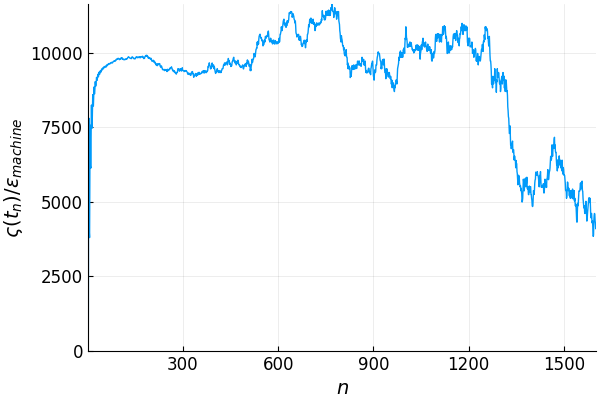
\includegraphics[width=0.8\linewidth]{simplecticity_pendulum}
 \caption{}
 \label{fig:simplecticity_pendulum}
\end{figure}

La figura \ref{fig:simplecticity_pendulum} muestra la variación de la cantidad $\varsigma(t)$ para el péndulo simple en términos de $\epsilon_{mahcine}$. Ésta se define como
\begin{equation}
 \varsigma(t) = \sum_{i,j} |\left[ J(\phi(t))^T \omega J(\phi(t)) - \omega \right]_{i,j}|
\end{equation}
y no es más que la suma de los valores absolutos de los elementos de matriz de (\ref{eq:sympletic_flow}). $\varsigma$ es una forma escalar de representar la simplecticidad del sistema para poder visualizarlo gráficamente para cada paso temporal.
  
Podemos observar en dicha figura un comportamiento browniano, similar a como pasa con la energía en los ejemplos de sistemas hamiltonianos planteados hasta ahora.


\subsection{Parametrización de parámetros}
\label{sec:parameter_variation}
Aunque el título de esta sección suene redundante, el TJ nos permite no sólo parametrizar las vecindades de $\xo$ en un campo vectorial dado sino también los parámetros que lo definen.

Tomemos, por ejemplo, al oscilador armónico\footnote{Al pobre oscilador armónico le deben picar las orejas de tanto que hablamos de él.} dado por  
\begin{equation}
 \ddot{x}(t) + \omega^2 x(t) = 0
 \label{eq:one_dim_oscil}
\end{equation}

cuyo hamiltoniano está dado por 
\begin{equation}
 H(x,y) = \frac{1}{2} \left( y^2 + \omega ^2 x^2 \right),
 \label{eq:osc_ham2}
\end{equation}
con $y = \dot{x}$.

Complejificando el dominio, sabemos que la solución está dada por 
\begin{equation*}
 x_{\mathbb{C}}(t) = A e^{i\omega t} + B e^{-i \omega t}
\end{equation*}
donde, si $\omega^2 < 0$, entonces la proyección a los reales es
\begin{equation}
 x(t) = a \cos(t) + b \sin (t)
 \label{eq:ho_solution_trig}
\end{equation}
y, si $\omega^2 > 0$, la proyección es
\begin{equation}
 x(t) = \alpha e^{\omega t} + \beta e^{- \omega t}.
 \label{eq:ho_solution_exp}
\end{equation}

%FIGURA!
\begin{figure}[h!]
 \centering
 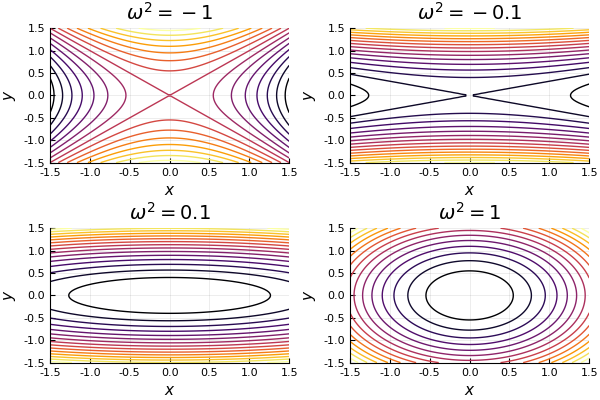
\includegraphics[width=0.8\linewidth]{oscillator_domega}
 \caption{Curvas de nivel dadas por (\ref{eq:osc_ham2}) para diferentes valores de $\omega^2$.}
 \label{fig:oscillator_domega}
\end{figure}

Observamos en la figura \ref{fig:oscillator_domega} cómo las curvas de nivel cambian para distintas $\omega^2$; en particular, observamos que las soluciones cambian de topología cuando $\omega^2$ cambia de signo. Con esto, pensar en una \textit{parametrización del parámetro} resulta una herramienta poderosa en el estudio de este tipo de sistemas ya que, por un lado, puede funcionar como un indicador para cambios de topología y, por otro, ayudar a encontrar conjuntos de soluciones cuando los parámetros no se conocen con exactitud. 

Para hacer esto con el transporte de jets, basta con incluir al parámetro o los parámetros que se quieran variar en el sistema de ecuaciones como $\dot{\lambda} = 0$, donde $\lambda$ es el conjunto de parámetros que se quieren variar. En este ejemplo el sistema queda como
\begin{align*}
 \dot{x} &= y \\
 \dot{y} &= - \omega^2 x \\
 \dot{\omega^2} &= 0
\end{align*}.
 
La figura \ref{fig:} muestra el trasnporte de jets para $\omega^2$ para una condición inicial, donde $\omega^2 = \omega_0^2 + \delta \xi$, con $\delta \xi$ la variación de $\omega^2$ dada por el transporte. 

%FIGURA! 
\begin{figure}[h!]
 \centering 
 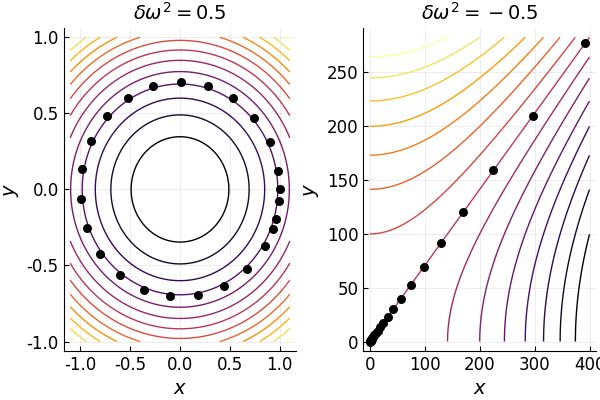
\includegraphics[width=0.8\linewidth]{oscillator_domega2}
 \caption{Solución para condición inicial $\xo = (1,0,0)$ y variación del parámetro para $\delta \omega^2 = 0.5$ en la izquierda y $-0.5$ en la derecha. $\delta \omega$ es un polinomio de orden $30$, y la expansión de Taylor para la solución es de orden $28$, con tolerancia de $10^{-20}$. Son $25$ pasos de integración de $0$ a $2 \pi$.}
\end{figure}

Resulta que el transporte de jets sí obtiene el cambio de topología dado por el signo de $\omega^2$. Sin embargo, hay que ver qué tan precisa es la solución, lo cual se puede checar con la conservación de la energía al evaluar el hamiltoniano. 

%FIGURA! 
\begin{figure}[h!]
 \centering
 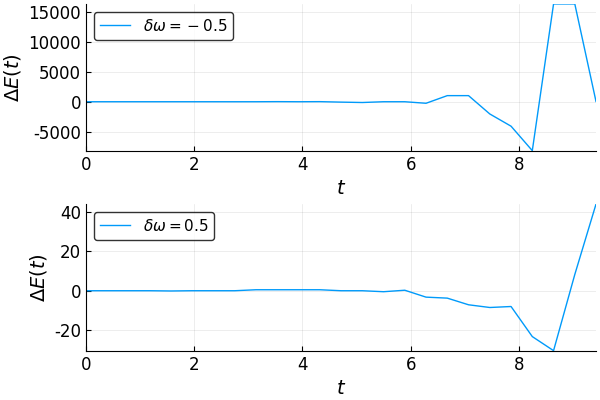
\includegraphics[width=0.8\linewidth]{oscillator_dE_domega}
 \caption{Variación $\Delta E = \frac{1}{\epsilon_{machine}} \left( E(t) - E_0 \right)$ de la energía respecto a la condición inicial para ambas evaluaciones del transporte $\delta \omega < 0$ y $\delta \omega > 0$.}
 \label{fig:oscillator_dE_domega}
\end{figure}

El flujo conserva la energía cada vez menos conforme pasa el tiempo como se observa en la figura \ref{fig:oscillator_dE_domega}; de hecho, la solución que diverge más pierde hasta $15000$ epsilons casi al final de la integración. Sin embargo, el error máximo en términos absolutos es de $3.63 \times 10^{-12}$, lo cual es bastante aceptable.

%Pequeña conclusión de sección ? 